\documentclass[11pt]{article}
\usepackage[a4paper,margin=1in]{geometry}
\usepackage[T1]{fontenc}
\usepackage{lmodern}
\usepackage{microtype}
\usepackage{amsmath,amssymb}
\usepackage{booktabs}
\usepackage{graphicx}
\usepackage{adjustbox}
\usepackage{float}
\usepackage[font=small,labelfont=bf]{caption}
\usepackage[numbers,sort&compress]{natbib}
\usepackage{xcolor}
\usepackage[colorlinks=true,linkcolor=blue!45!black,citecolor=blue!45!black,urlcolor=blue!45!black]{hyperref}
\graphicspath{{../results/figures/}}
% Generated by `python -m eval.paper_numbers` from the committed results. Do not edit.
\newcommand{\ProtoHash}{\texttt{c97977a4a4bbb055}}
\newcommand{\PathStart}{2018-12-31}
\newcommand{\PathEnd}{2026-11-06}
\newcommand{\NSessions}{$1{,}936$}
\newcommand{\NCaptures}{$76$}
\newcommand{\NMemberSets}{$19$}
\newcommand{\NChanges}{$78$}
\newcommand{\NChangeDates}{$25$}
\newcommand{\NSnapMatch}{$67$}
\newcommand{\NSnap}{$68$}
\newcommand{\NSymbols}{$87$}
\newcommand{\NPriced}{$81$}
\newcommand{\NExcluded}{$6$}
\newcommand{\ExcludedList}{CAIRN, HDFC, IDFC, JPASSOCIAT, RANBAXY, TATAMTRDVR}
\newcommand{\EligMin}{$45$}
\newcommand{\EligMed}{$49$}
\newcommand{\EligMax}{$50$}
\newcommand{\NRepairs}{$4$}
\newcommand{\NBenchRepairs}{$3$}
\newcommand{\NBenchGaps}{$3$}
\newcommand{\RfMin}{$2.93\%$}
\newcommand{\RfMax}{$7.05\%$}
\newcommand{\RfMean}{$5.33\%$}
\newcommand{\FreezeDate}{2026-11-06}
\newcommand{\RunMinutesMean}{$2.7$}
\newcommand{\ValTwentyMin}{$-0.15$}
\newcommand{\ValTwentyMax}{$-0.07$}
\newcommand{\HiDelta}{$+0.320$}
\newcommand{\HiPfive}{$+0.054$}
\newcommand{\HiLo}{$+0.000$}
\newcommand{\HiHi}{$+0.620$}
\newcommand{\HiShare}{$2.5\%$}
\newcommand{\SRppo}{$0.808$}
\newcommand{\CAGRppo}{$14.9\%$}
\newcommand{\VOLppo}{$11.4\%$}
\newcommand{\MDDppo}{$-20.7\%$}
\newcommand{\CALppo}{$0.72$}
\newcommand{\COSTppo}{$2.7\%$}
\newcommand{\EXPppo}{$0.66$}
\newcommand{\SRvt}{$0.488$}
\newcommand{\CAGRvt}{$11.4\%$}
\newcommand{\VOLvt}{$12.9\%$}
\newcommand{\MDDvt}{$-29.9\%$}
\newcommand{\CALvt}{$0.38$}
\newcommand{\COSTvt}{$2.7\%$}
\newcommand{\EXPvt}{$0.87$}
\newcommand{\SRvtu}{$0.483$}
\newcommand{\CAGRvtu}{$11.5\%$}
\newcommand{\VOLvtu}{$13.5\%$}
\newcommand{\MDDvtu}{$-29.9\%$}
\newcommand{\CALvtu}{$0.39$}
\newcommand{\COSTvtu}{$2.8\%$}
\newcommand{\EXPvtu}{$0.93$}
\newcommand{\SRbest}{$0.547$}
\newcommand{\CAGRbest}{$12.2\%$}
\newcommand{\VOLbest}{$12.9\%$}
\newcommand{\MDDbest}{$-34.9\%$}
\newcommand{\CALbest}{$0.35$}
\newcommand{\COSTbest}{$2.0\%$}
\newcommand{\EXPbest}{$0.65$}
\newcommand{\SRew}{$0.662$}
\newcommand{\CAGRew}{$16.4\%$}
\newcommand{\VOLew}{$17.2\%$}
\newcommand{\MDDew}{$-38.3\%$}
\newcommand{\CALew}{$0.43$}
\newcommand{\COSTew}{$1.2\%$}
\newcommand{\EXPew}{$1.00$}
\newcommand{\SRbees}{$0.503$}
\newcommand{\CAGRbees}{$12.7\%$}
\newcommand{\VOLbees}{$15.5\%$}
\newcommand{\MDDbees}{$-36.3\%$}
\newcommand{\CALbees}{$0.35$}
\newcommand{\COSTbees}{$0.1\%$}
\newcommand{\EXPbees}{$1.00$}
\newcommand{\SRrpA}{$0.624$}
\newcommand{\CAGRrpA}{$10.4\%$}
\newcommand{\VOLrpA}{$7.8\%$}
\newcommand{\MDDrpA}{$-17.4\%$}
\newcommand{\CALrpA}{$0.60$}
\newcommand{\COSTrpA}{$0.8\%$}
\newcommand{\EXPrpA}{$0.50$}
\newcommand{\SRrpB}{$0.619$}
\newcommand{\CAGRrpB}{$12.2\%$}
\newcommand{\VOLrpB}{$11.0\%$}
\newcommand{\MDDrpB}{$-24.3\%$}
\newcommand{\CALrpB}{$0.50$}
\newcommand{\COSTrpB}{$1.2\%$}
\newcommand{\EXPrpB}{$0.70$}
\newcommand{\SRrpC}{$0.615$}
\newcommand{\CAGRrpC}{$13.5\%$}
\newcommand{\VOLrpC}{$13.4\%$}
\newcommand{\MDDrpC}{$-29.7\%$}
\newcommand{\CALrpC}{$0.45$}
\newcommand{\COSTrpC}{$1.6\%$}
\newcommand{\EXPrpC}{$0.85$}
\newcommand{\SRrpD}{$0.611$}
\newcommand{\CAGRrpD}{$14.7\%$}
\newcommand{\VOLrpD}{$15.8\%$}
\newcommand{\MDDrpD}{$-35.0\%$}
\newcommand{\CALrpD}{$0.42$}
\newcommand{\COSTrpD}{$2.0\%$}
\newcommand{\EXPrpD}{$1.00$}
\newcommand{\SRseedMin}{$0.611$}
\newcommand{\SRseedMax}{$0.876$}
\newcommand{\NSeedsBeatVT}{5}
\newcommand{\SRppoLag}{$0.808$}
\newcommand{\SRvtLag}{$0.532$}
\newcommand{\SRppoCost}{$0.791$}
\newcommand{\SRvtCost}{$0.470$}
\newcommand{\SRewCost}{$0.656$}
\newcommand{\MDDppoLag}{$-22.8\%$}
\newcommand{\SRrand}{$0.567$}
\newcommand{\SRrandLo}{$0.410$}
\newcommand{\SRrandHi}{$0.759$}
\newcommand{\DSRthis}{$0.987$}
\newcommand{\DSRthisN}{1}
\newcommand{\DSRprior}{$0.412$}
\newcommand{\DSRpriorN}{83}
\newcommand{\SRdaily}{$0.0509$}
\newcommand{\Kurt}{$20.4$}
\newcommand{\Skew}{$+0.05$}
\newcommand{\DSRnow}{$0.957$}
\newcommand{\DSRnowN}{2}
\newcommand{\DSRpriorNow}{$0.410$}
\newcommand{\DSRpriorNowN}{84}
\newcommand{\SecMddEW}{$+0.176$}
\newcommand{\SecMddEWCI}{[$+0.041$, $+0.249$]}
\newcommand{\SecMddEWpp}{$+17.6$}
\newcommand{\SecMddEWppCI}{[$+4.1$, $+24.9$]}
\newcommand{\SecCalEW}{$+0.292$}
\newcommand{\SecCalEWCI}{[$+0.050$, $+0.808$]}
\newcommand{\SecMddBees}{$+0.157$}
\newcommand{\SecMddBeesCI}{[$+0.032$, $+0.278$]}
\newcommand{\SecMddBeespp}{$+15.7$}
\newcommand{\SecMddBeesppCI}{[$+3.2$, $+27.8$]}
\newcommand{\SecCalBees}{$+0.373$}
\newcommand{\SecCalBeesCI}{[$+0.098$, $+1.151$]}
\newcommand{\NYearsAhead}{5}
\newcommand{\NYears}{8}
\newcommand{\DeltaTwenty}{$+1.175$}
\newcommand{\DeltaTwentyCI}{[$-0.117$, $+1.847$]}
\newcommand{\DvsBest}{$+0.261$}
\newcommand{\DvsBestCI}{[$-0.149$, $+0.550$]}
\newcommand{\DvsEW}{$+0.147$}
\newcommand{\DvsEWCI}{[$-0.078$, $+0.345$]}
\newcommand{\DvsBees}{$+0.305$}
\newcommand{\DvsBeesCI}{[$-0.041$, $+0.608$]}
\newcommand{\DvsRpB}{$+0.190$}
\newcommand{\DvsRpBCI}{[$-0.015$, $+0.379$]}
\newcommand{\EpiPPO}{$-20.0\%$}
\newcommand{\EpiVT}{$-29.1\%$}
\newcommand{\EpiEW}{$-36.7\%$}
\newcommand{\EpiBees}{$-36.3\%$}
\newcommand{\EpiPeak}{2020-01-17}
\newcommand{\EpiTrough}{2020-03-23}
\newcommand{\EpiTwentyFiveBees}{$-2.1\%$}
\newcommand{\DeepThreePeak}{2024-09-27}
\newcommand{\DeepThreeTrough}{2025-03-04}
\newcommand{\DeepThreePPO}{$-8.9\%$}
\newcommand{\DeepThreeVT}{$-18.6\%$}
\newcommand{\DeepThreeBees}{$-15.2\%$}
\newcommand{\CrashDecisions}{$0.50$ on 29 January; $0.60$ on 28 February; $1.00$ on 31 March}
\newcommand{\CrashDiffDate}{28 February 2020}
\newcommand{\PPOCrashExp}{$0.60$}
\newcommand{\VRCrashExp}{$1.00$}
\newcommand{\VixCrash}{$23.2$}
\newcommand{\NCrashDates}{3}
\newcommand{\ExNoDelta}{$+0.101$}
\newcommand{\ExNoPfive}{$-0.149$}
\newcommand{\ExNoCI}{[$-0.194$, $+0.400$]}
\newcommand{\ExNoPPO}{$0.649$}
\newcommand{\ExNoVT}{$0.548$}
\newcommand{\ExSeenDelta}{$+0.045$}
\newcommand{\ExSeenPfive}{$-0.260$}
\newcommand{\ExSeenCI}{[$-0.316$, $+0.413$]}
\newcommand{\ExSeenPPO}{$0.487$}
\newcommand{\ExSeenVT}{$0.443$}
\newcommand{\ExUnseenDelta}{$+0.607$}
\newcommand{\ExUnseenPfive}{$+0.114$}
\newcommand{\ExUnseenCI}{[$+0.017$, $+1.055$]}
\newcommand{\ExUnseenPPO}{$1.162$}
\newcommand{\ExUnseenVT}{$0.555$}
\newcommand{\ExNoEW}{$0.691$}
\newcommand{\ExpLowVix}{$0.54$}
\newcommand{\ExpHighVix}{$0.87$}
\newcommand{\FloorShareLowVix}{$71\%$}
\newcommand{\CorrVix}{$+0.62$}
\newcommand{\CorrDD}{$-0.29$}
\newcommand{\NDecisions}{$118$}
\newcommand{\VRsr}{$0.658$}
\newcommand{\VRdelta}{$+0.151$}
\newcommand{\VRpfive}{$-0.176$}
\newcommand{\VRci}{[$-0.220$, $+0.417$]}
\newcommand{\VRvsVT}{$+0.169$}
\newcommand{\VRvsVTci}{[$-0.122$, $+0.535$]}
\newcommand{\VRnoRule}{$0.742$}
\newcommand{\VRnoPPO}{$0.649$}
\newcommand{\VRmdd}{$-30.6\%$}
\newcommand{\VRtwentyRule}{$0.841$}
\newcommand{\VRtwentyPPO}{$1.491$}
\newcommand{\VRcorr}{$+0.37$}
\newcommand{\NxProtoHash}{\texttt{217c789dd2a95d9d}}
\newcommand{\NxPathStart}{2018-12-31}
\newcommand{\NxPathEnd}{2026-11-06}
\newcommand{\NxSessions}{$1{,}936$}
\newcommand{\NxAlpha}{$0.05$}
\newcommand{\NxHOneDelta}{$+0.195$}
\newcommand{\NxHOneCI}{[$-0.088$, $+0.447$]}
\newcommand{\NxHOneP}{$0.085$}
\newcommand{\NxHOneThr}{$0.025$}
\newcommand{\NxHTwoDelta}{$-0.028$}
\newcommand{\NxHTwoCI}{[$-0.325$, $+0.213$]}
\newcommand{\NxHTwoP}{$0.613$}
\newcommand{\NxHTwoThr}{$0.050$}
\newcommand{\NxSRppo}{$0.639$}
\newcommand{\NxCAGRppo}{$13.8\%$}
\newcommand{\NxVOLppo}{$13.3\%$}
\newcommand{\NxMDDppo}{$-27.5\%$}
\newcommand{\NxCALppo}{$0.50$}
\newcommand{\NxEXPppo}{$0.73$}
\newcommand{\NxSRvt}{$0.444$}
\newcommand{\NxCAGRvt}{$11.0\%$}
\newcommand{\NxVOLvt}{$13.6\%$}
\newcommand{\NxMDDvt}{$-33.8\%$}
\newcommand{\NxCALvt}{$0.33$}
\newcommand{\NxEXPvt}{$0.78$}
\newcommand{\NxSRvtu}{$0.413$}
\newcommand{\NxCAGRvtu}{$10.7\%$}
\newcommand{\NxVOLvtu}{$14.2\%$}
\newcommand{\NxMDDvtu}{$-33.8\%$}
\newcommand{\NxCALvtu}{$0.32$}
\newcommand{\NxEXPvtu}{$0.87$}
\newcommand{\NxSRvix}{$0.667$}
\newcommand{\NxCAGRvix}{$13.6\%$}
\newcommand{\NxVOLvix}{$12.3\%$}
\newcommand{\NxMDDvix}{$-30.0\%$}
\newcommand{\NxCALvix}{$0.45$}
\newcommand{\NxEXPvix}{$0.61$}
\newcommand{\NxSRbest}{$0.507$}
\newcommand{\NxCAGRbest}{$10.3\%$}
\newcommand{\NxVOLbest}{$9.7\%$}
\newcommand{\NxMDDbest}{$-17.2\%$}
\newcommand{\NxCALbest}{$0.60$}
\newcommand{\NxEXPbest}{$0.53$}
\newcommand{\NxSRew}{$0.552$}
\newcommand{\NxCAGRew}{$14.9\%$}
\newcommand{\NxVOLew}{$18.7\%$}
\newcommand{\NxMDDew}{$-37.0\%$}
\newcommand{\NxCALew}{$0.40$}
\newcommand{\NxEXPew}{$1.00$}
\newcommand{\NxSRbees}{$0.514$}
\newcommand{\NxCAGRbees}{$13.6\%$}
\newcommand{\NxVOLbees}{$17.4\%$}
\newcommand{\NxMDDbees}{$-34.5\%$}
\newcommand{\NxCALbees}{$0.39$}
\newcommand{\NxEXPbees}{$1.00$}
\newcommand{\NxSRrpA}{$0.602$}
\newcommand{\NxCAGRrpA}{$10.5\%$}
\newcommand{\NxVOLrpA}{$8.3\%$}
\newcommand{\NxMDDrpA}{$-17.2\%$}
\newcommand{\NxCALrpA}{$0.61$}
\newcommand{\NxEXPrpA}{$0.50$}
\newcommand{\NxSRrpB}{$0.600$}
\newcommand{\NxCAGRrpB}{$12.4\%$}
\newcommand{\NxVOLrpB}{$11.7\%$}
\newcommand{\NxMDDrpB}{$-24.0\%$}
\newcommand{\NxCALrpB}{$0.52$}
\newcommand{\NxEXPrpB}{$0.70$}
\newcommand{\NxSRrpC}{$0.598$}
\newcommand{\NxCAGRrpC}{$13.7\%$}
\newcommand{\NxVOLrpC}{$14.3\%$}
\newcommand{\NxMDDrpC}{$-28.9\%$}
\newcommand{\NxCALrpC}{$0.47$}
\newcommand{\NxEXPrpC}{$0.85$}
\newcommand{\NxSRrpD}{$0.596$}
\newcommand{\NxCAGRrpD}{$15.0\%$}
\newcommand{\NxVOLrpD}{$16.9\%$}
\newcommand{\NxMDDrpD}{$-33.8\%$}
\newcommand{\NxCALrpD}{$0.44$}
\newcommand{\NxEXPrpD}{$1.00$}
\newcommand{\NxSRrpMin}{$0.596$}
\newcommand{\NxSRrpMax}{$0.602$}
\newcommand{\NxSRseedMin}{$0.559$}
\newcommand{\NxSRseedMax}{$0.770$}
\newcommand{\NxNSeedsBeatVT}{5}
\newcommand{\NxNSeedsBeatVix}{1}
\newcommand{\NxSRppoLag}{$0.626$}
\newcommand{\NxSRvtLag}{$0.461$}
\newcommand{\NxSRvixLag}{$0.662$}
\newcommand{\NxSRppoCost}{$0.622$}
\newcommand{\NxSRvtCost}{$0.427$}
\newcommand{\NxSRvixCost}{$0.649$}
\newcommand{\NxSRrand}{$0.538$}
\newcommand{\NxSRrandLo}{$0.383$}
\newcommand{\NxSRrandHi}{$0.688$}
\newcommand{\NxDSRthis}{$0.813$}
\newcommand{\NxDSRthisN}{3}
\newcommand{\NxDSRprior}{$0.248$}
\newcommand{\NxDSRpriorN}{85}
\newcommand{\NxSecMddEWpp}{$+9.5$}
\newcommand{\NxSecMddEWppCI}{[$+4.3$, $+18.6$]}
\newcommand{\NxSecCalEW}{$+0.100$}
\newcommand{\NxSecCalEWCI}{[$-0.043$, $+0.539$]}
\newcommand{\NxSecMddBeespp}{$+7.0$}
\newcommand{\NxSecMddBeesppCI}{[$+3.9$, $+20.0$]}
\newcommand{\NxSecCalBees}{$+0.109$}
\newcommand{\NxSecCalBeesCI}{[$-0.022$, $+0.671$]}
\newcommand{\NxNYears}{8}
\newcommand{\NxNYearsAheadVT}{8}
\newcommand{\NxNYearsAheadVix}{3}
\newcommand{\NxYearsCIpos}{2019 and 2026}
\newcommand{\NxDeltaTwenty}{$+0.758$}
\newcommand{\NxDeltaTwentyCI}{[$-0.068$, $+1.314$]}
\newcommand{\NxDeltaVixTwenty}{$+0.151$}
\newcommand{\NxEpiPeak}{2020-01-24}
\newcommand{\NxEpiTrough}{2020-03-24}
\newcommand{\NxEpiPPO}{$-26.8\%$}
\newcommand{\NxEpiVT}{$-33.0\%$}
\newcommand{\NxEpiVix}{$-29.2\%$}
\newcommand{\NxEpiEW}{$-36.5\%$}
\newcommand{\NxEpiBees}{$-34.5\%$}
\newcommand{\NxEpiBest}{$-16.8\%$}
\newcommand{\NxBeesPeak}{27 September 2024}
\newcommand{\NxCorrVix}{$+0.42$}
\newcommand{\NxNDecisions}{$97$}
\newcommand{\NxExpLowVix}{$0.67$}
\newcommand{\NxExpHighVix}{$0.92$}
\newcommand{\NxRunMinutes}{$2.6$}
\newcommand{\NxValTwentyMin}{$-0.15$}
\newcommand{\NxValTwentyMax}{$-0.05$}
\newcommand{\NxNotices}{$449$}
\newcommand{\NxNoticesUsed}{$38$}
\newcommand{\NxReviews}{$26$}
\newcommand{\NxAdHoc}{$12$}
\newcommand{\NxChanges}{$308$}
\newcommand{\NxChangeDates}{$37$}
\newcommand{\NxReadings}{$37$}
\newcommand{\NxReadingsMatch}{$37$}
\newcommand{\NxReadingsNext}{$22$}
\newcommand{\NxReadingsHundred}{$15$}
\newcommand{\NxCopies}{$36$}
\newcommand{\NxCopiesSame}{$34$}
\newcommand{\NxSymbols}{$152$}
\newcommand{\NxPriced}{$143$}
\newcommand{\NxExcluded}{$9$}
\newcommand{\NxExcludedList}{ABIRLANUVO, CAIRN, GSKCONS, ICICIPRULI, INGVYSYABK, MINDTREE, PEL, RANBAXY, RELCAPITAL}
\newcommand{\NxExclShare}{$2.8\%$}
\newcommand{\NxJumps}{$13$}
\newcommand{\NxJumpsOK}{$13$}
\newcommand{\NxBenchRepairs}{$1$}
\newcommand{\NxBenchGaps}{$6$}
\newcommand{\NxEligMin}{$45$}
\newcommand{\NxEligMed}{$48$}
\newcommand{\NxEligMax}{$50$}
\newcommand{\NxCorrDev}{$0.83$}
\newcommand{\NxRepairs}{$4$}
\newcommand{\NxSplitRepairs}{$3$}
\newcommand{\NxBadRepairSym}{CONCOR}
\newcommand{\NxBadRepairDate}{4 June 2024}
\newcommand{\NxBadRepairNSE}{$-19.2\%$}
\newcommand{\NxBadRepairRep}{$+1.0\%$}

\newcommand{\figwidth}{\linewidth}
\newcommand{\gtab}[1]{\begin{adjustbox}{max width=\linewidth}\input{generated/#1}\end{adjustbox}}

\title{Reinforcement Learning as a Risk-Budget Controller:\\
A Pre-Registered Walk-Forward Test on Point-in-Time Nifty~50 Equities}
\author{Eshani Parulekar \and Dhruv Pande \and Rishaan Damani\\[2pt]
\small Plaksha University}
\date{\small Working draft, \today. Every number is generated from the committed results by \texttt{python -m eval.paper\_numbers}.}

\begin{document}
\maketitle

\begin{abstract}
In our earlier study, a Proximal Policy Optimization (PPO) agent that chose the risk aversion and holding horizon of a mean-variance optimiser on seven Indian stocks lost to a passive index fund out of sample. Here we move the agent from return forecasting to risk control. The agent chooses only the exposure (50 to 100 per cent) and rebalance horizon (5 or 21 sessions) of an equal-risk-contribution portfolio drawn from a point-in-time Nifty~50 universe, and cash earns the Reserve Bank of India's 91-day Treasury-bill rate. Before any test year was scored we registered the protocol: walk-forward folds with test years 2019 to 2026, five seeds per fold combined in an ensemble, a common simulation engine for every strategy, and a single primary hypothesis against volatility targeting. In the single test run (\NSessions{} sessions), the ensemble's Sharpe ratio was \SRppo{} against \SRvt{} for volatility targeting, and the 5th percentile of the paired block-bootstrap difference was \HiPfive{}, so the hypothesis is supported. The deflated Sharpe ratio is \DSRnow{} counting this study's \DSRnowN{} trials and \DSRpriorNow{} once the \DSRpriorNowN{} trials recorded across our earlier work are included. Analyses made after the test qualify the result. The margin comes from the 2020 crash and recovery; the agent learned to raise exposure when India VIX is high, the opposite of volatility targeting; and a two-parameter VIX threshold rule fixed after the test cannot be distinguished from the agent. We read the evidence as a narrow pre-registered win whose economic content is contrarian volatility timing.
\end{abstract}

\section{Introduction}

Reinforcement learning (RL) has been applied to trading and portfolio choice for more than two decades \citep{moody1998,moody2001,deng2017,jiang2017,zhang2020drl,yang2020ensemble,liu2020finrl}; \citet{hambly2023} and \citet{pippas2024} survey the field. Published backtests in this area are hard to compare and easy to overstate. Look-ahead in features or execution, universes chosen with hindsight, single training seeds, missing costs and an unreported number of tried configurations can each manufacture an apparent edge \citep{brown1992,bailey2014notices,henderson2018,lopezdeprado2018}.

Our own earlier study is a case in point \citep{parulekar2026}. A PPO agent chose the risk-aversion coefficient and holding horizon of a long-only mean-variance optimiser on seven large Indian stocks. Once the trading clock, data splits and costs were corrected, the agent lost to the NIFTYBEES index fund on its 2025--2026 forward period: a mean Sharpe ratio of $-1.72$ across seeds against $-0.67$ for the fund. A controller whose decisions depend on forecasting returns did not work.

This paper moves the agent from return forecasting to risk control. The agent never forecasts individual stocks. It decides how much of an equal-risk-contribution (ERC) portfolio to hold, between half and all of it, and how long to wait before deciding again. Three things recommend this design. Risk is more predictable than returns, which is the premise of volatility timing \citep{fleming2001,moreira2017}. A strong rule already answers the same question, volatility targeting \citep{harvey2018vt}, which gives the agent a demanding and interpretable comparator. And a small discrete action space keeps the policy auditable.

We built the test to be hard to fool. The Nifty~50 universe is rebuilt point in time from archived copies of the exchange's own constituent files. Cash earns the Treasury-bill rate of each date. The protocol, including the single primary hypothesis, was registered and tagged in version control before any test year was scored, and every training run and analysis is recorded in an append-only trial ledger. Models are trained walk-forward, one fold per test year from 2019 to 2026, with five seeds per fold. Test years 2022 to 2026 are flagged as previously seen, because our earlier work used them.

The pre-registered hypothesis is supported, but narrowly. The ensemble's Sharpe ratio exceeds that of volatility targeting by \HiDelta{}, with a bootstrap 5th percentile of \HiPfive{}. The result survives a one-session execution delay and doubled costs, and all five seeds beat volatility targeting on their own. Analyses made after the test, which we label exploratory, show where the margin comes from. Most of it is earned in 2020. The agent learned to hold little exposure when India VIX is low and to raise exposure after VIX spikes. A simple VIX threshold rule, designed after the test, cannot be distinguished from it.

Our contributions are:
\begin{itemize}
\item a pre-registered walk-forward evaluation of an RL risk-budget controller on a point-in-time Nifty~50 panel, with code, data hashes and a trial ledger;
\item evidence that the controller beats volatility targeting under the registered test, reported with intervals, seed-level results and deflated Sharpe ratios that count earlier trials; and
\item an exploratory decomposition of that result: what the agent learned, where its margin comes from, and a simple rule that matches it.
\end{itemize}
Section~\ref{sec:related} reviews related work, Section~\ref{sec:data} the data and Section~\ref{sec:method} the method. Section~\ref{sec:protocol} sets out the registered evaluation, Section~\ref{sec:results} its results and Section~\ref{sec:exploratory} the exploratory analyses. Section~\ref{sec:discussion} discusses limitations.

\section{Related work}\label{sec:related}

\paragraph{Reinforcement learning for trading and portfolios.} Direct reinforcement for trading began with \citet{moody1998} and \citet{moody2001}; deep variants followed \citep{deng2017,jiang2017,zhang2020drl}, as did ensembles of agents \citep{yang2020ensemble} and open libraries \citep{liu2020finrl}. A related line keeps a conventional optimiser in the loop and lets learning steer it: RL over mean-variance optimisation \citep{pretorius2022,sood2023}, and end-to-end risk budgeting with neural networks \citep{uysal2024}. \citet{sen2023} compare mean-variance, hierarchical risk parity and RL on Indian equities. Our agent is a controller of this hybrid kind, restricted to the risk budget. Because it also chooses how long each decision lasts, its actions are temporally extended in the sense of semi-Markov options \citep{sutton1999options}.

\paragraph{Volatility timing and targeting.} \citet{fleming2001} show that timing volatility has economic value, and \citet{moreira2017} report that scaling exposure by inverse recent variance raises Sharpe ratios across many factors. \citet{harvey2018vt} find that volatility targeting mainly reduces tail risk, with Sharpe gains concentrated in risk assets. Out of sample the evidence is weaker: \citet{cederburg2020} find that volatility-managed portfolios do not systematically beat their unmanaged versions. Our primary comparator is volatility targeting with a 50 per cent exposure floor, matching the agent's own floor.

\paragraph{Risk parity and diversification.} The ERC portfolio equalises each asset's contribution to portfolio risk \citep{maillard2010}. We compute it with the convex formulation of \citet{spinu2013} on the shrinkage covariance estimator of \citet{ledoit2004}. Naive diversification is a hard benchmark to beat \citep{demiguel2009}, so equal weight is among our baselines.

\paragraph{Evaluation practice.} Sharpe ratios are noisy and serially dependent \citep{lo2002}; we compare them with a paired block bootstrap \citep{politis1992,ledoit2008}. Selecting the best of many backtests inflates performance \citep{bailey2014notices,harvey2016}; the probabilistic and deflated Sharpe ratios correct for non-normality and for the number of trials \citep{bailey2012psr,bailey2014dsr}. In RL, results vary widely across seeds \citep{henderson2018}, and point estimates without intervals mislead \citep{agarwal2021}. Pre-registration, standard in other empirical fields, commits the analysis before the data can shape it \citep{nosek2018}.

\section{Data}\label{sec:data}

\paragraph{Universe.} We rebuilt Nifty~50 membership from \NCaptures{} archived captures of the National Stock Exchange's constituent files and index API, held by the Internet Archive, which contain \NMemberSets{} distinct member sets. Between captures, \NChanges{} additions and removals on \NChangeDates{} effective dates are dated from exchange notices or news reports, and renamed securities are linked by ISIN. The rebuilt roster matches \NSnapMatch{} of the \NSnap{} snapshots taken on or after 1~January 2014; the one mismatch is a stale copy of the file from before a rename. The index has exactly 50 members on every session, or 51 while the Tata Motors DVR share was an additional security (April 2016 to September 2017).

\paragraph{Prices.} Daily adjusted closes come from Yahoo Finance. Of the \NSymbols{} symbols that were members between 2014 and the data freeze, \NPriced{} have usable series. The other \NExcluded{} (\ExcludedList) have none and are excluded while members; the largest is HDFC, a member until its merger in July 2023. A stock is eligible on a session when it is a member for the next session, has a price and has a complete 120-session return history; between \EligMin{} and \EligMax{} stocks are eligible on each session (median \EligMed{}). We repaired \NRepairs{} corporate-action errors, three demergers and one split-adjustment artifact, each from the exchange's own prices (Appendix~\ref{app:data}).

\paragraph{Benchmark, market series and cash.} NIFTYBEES, an exchange-traded fund on the Nifty~50, is the passive benchmark, using its adjusted close as a total-return series; \NBenchRepairs{} sessions with vendor errors are repaired and \NBenchGaps{} genuine tracking gaps are kept. The Nifty~50 index, India VIX and the rupee-dollar rate (lagged one session, because its close falls after the exchange's) feed the agent's state. Cash earns the cut-off yield of the RBI's weekly 91-day Treasury-bill auctions \citep{rbi91}: each yield applies from the session after its auction and accrues as $(1+y)^{d/365}-1$ over $d$ calendar days. Over the test path the yield ranged from \RfMin{} to \RfMax{} (mean \RfMean{}).

\paragraph{Calendar and freeze.} A session is any date with a Nifty~50 close on Yahoo Finance. This calendar skips a few exchange sessions, such as 1~January 2019, and a return then spans the skipped day; no return is lost. The data are frozen at the last session on or before \FreezeDate{}, and every raw and processed file is listed with its SHA-256 hash.

\section{Method}\label{sec:method}

\subsection{Allocator and engine}

On each session $t$ the allocator computes ERC weights $w_t$ over the eligible stocks from the Ledoit-Wolf covariance $\Sigma_t$ of the trailing 120 daily returns. Following \citet{spinu2013}, it solves
\begin{equation}
y^\star = \arg\min_{y>0}\ \tfrac{1}{2}\,y^\top \Sigma_t\, y - \tfrac{1}{N}\sum_{i=1}^{N} \log y_i, \qquad w_t = y^\star / \mathbf{1}^\top y^\star,
\end{equation}
whose solution gives each stock the same contribution $w_i(\Sigma_t w)_i$ to portfolio variance. The weights do not depend on the agent's actions, so they are computed once for every session.

All strategies run on one engine. A decision at the close of session $t$ sets the stock book to $e_t w_t$ of net asset value and holds $1-e_t$ in cash; trades execute at that close and returns accrue from session $t+1$. Each trade costs 10 basis points of the value traded. Holdings drift between decisions. A stock that leaves the index is sold at the close of its last member session. A decision is forced at each year-end close, so every test year is traded only by its own fold's models.

\subsection{Agent}

At each decision the agent picks an exposure $e \in \{0.5, 0.7, 0.85, 1.0\}$ and a horizon $h \in \{5, 21\}$ sessions until its next decision. Its reward for the interval is
\begin{equation}
R = 100\left[\sum_{\tau=t+1}^{t+h} \bigl(\log(1+r_\tau) - \log(1+r^f_\tau)\bigr) - \kappa \max\bigl(0,\ D_{t+h} - D_t\bigr)\right],
\end{equation}
where $r_\tau$ is the strategy's return net of costs, $r^f_\tau$ the cash return, $D$ the magnitude of the strategy's drawdown from its running peak and $\kappa=1$. The state has 13 features. Ten describe the market: Nifty~50 realised volatility over 20 and 60 sessions and their ratio; index momentum over 21 and 63 sessions; the index drawdown from its 252-session high; the average pairwise correlation of eligible stocks over 60 sessions; the India VIX level and its five-session log change; and the 21-session change in the rupee-dollar rate. These are standardised with the mean and standard deviation of the fold's training years only and clipped at $\pm 5$. Three describe the agent's own portfolio: its current exposure, drawdown and 20-session volatility.

We train with PPO \citep{schulman2017ppo} in Stable-Baselines3 \citep{raffin2021sb3}, using a $64\times 64$ network, learning rate $3\times 10^{-4}$, 1{,}024 steps per update, minibatches of 64, ten epochs, discount 1, generalised advantage estimation with $\lambda = 0.95$ \citep{schulman2016gae}, clip range 0.2 and entropy coefficient 0.01. Training episodes are random 252-session windows within the training years, each starting in cash.

\subsection{Walk-forward folds and the ensemble}

Each test year $Y$ from 2019 to 2026 has its own fold: training on 2014 to $Y-3$ and validation on $Y-2$ and $Y-1$ (Appendix~\ref{app:folds}). Each fold trains five seeds for 200{,}000 steps. Every 10{,}000 steps the current policy is run deterministically on each validation year, starting from cash, and the checkpoint with the best mean Sharpe ratio over the two years is kept. A run took \RunMinutesMean{} minutes on average on a laptop CPU. The ensemble keeps its own portfolio and state; at each of its decisions it queries all five seeds, takes the mean of their exposures and the median of their horizons.

\subsection{Baselines}

Every baseline uses the same engine, costs and execution, and starts in cash at the last close of 2018:
NIFTYBEES bought and held;
equal weight over eligible stocks, rebalanced at each month end;
risk parity at a fixed exposure of 0.5, 0.7, 0.85 or 1.0, rebalanced every 21 sessions;
the best fixed action, chosen per fold on validation;
a random policy over the agent's eight actions (100 seeds); and
volatility targeting. Volatility targeting sets $e_t = \mathrm{clip}(\tau/\hat\sigma_t,\ 0.5,\ 1)$, where $\hat\sigma_t$ is the realised volatility of the unlevered ERC portfolio over 60 sessions; the target $\tau \in \{10, 12, 15\}$ per cent and horizon $h \in \{5, 21\}$ are chosen per fold on validation by the same criterion as the agent's checkpoints. The same rule without the floor is a secondary baseline.

\section{Pre-registered evaluation}\label{sec:protocol}

\paragraph{Registration.} The protocol (\texttt{protocol.md}, mirrored by \texttt{config/protocol.yaml}, SHA-256 prefix \ProtoHash{}) was signed by all three authors and tagged \texttt{protocol-v1} on 7~November 2026, before any test year was scored. The test script refuses to run unless the tag exists, the configuration is unchanged since the tag, the working tree is clean and the cash series is the RBI one, and it writes its ledger entry before computing any test-year score. It was run once.

\paragraph{Primary hypothesis.} H1: the PPO ensemble's Sharpe ratio exceeds that of floored volatility targeting over the combined test path. Sharpe ratios are annualised: $\sqrt{252}$ times the mean daily excess return over its standard deviation. We resample the paired daily returns of the two strategies with a circular block bootstrap \citep{politis1992} in blocks of 20 sessions, 10{,}000 times with a fixed seed. H1 is supported if the 5th percentile of the bootstrapped Sharpe difference is above zero.

\paragraph{Secondary outcomes and sensitivities.} The secondary outcomes are maximum drawdown and Calmar ratio against equal weight and NIFTYBEES. Four sensitivities were registered: executing every trade one session late, doubling costs to 20 basis points, the unfloored volatility rule, and a 30 per cent loss on any stock that stopped trading while a member (none did on the test path, so it does not apply). Every other comparison is exploratory.

\paragraph{Multiple testing.} We report the deflated Sharpe ratio (DSR) of \citet{bailey2014dsr}: the probability that the true Sharpe ratio exceeds the expected maximum of $N$ unskilled trials, with the null variance of the Sharpe ratio set to $1/(T-1)$ and the non-normality correction of \citet{bailey2012psr}. $N$ is taken from the ledger, once for this study alone and once including the trials of our earlier work (Appendix~\ref{app:ledger}).

\paragraph{Correctness checks.} Before any training, the test suite established that perturbing every series after a date leaves all features, weights, standardisation statistics, decisions and net asset values before it bit-identical; that an oracle policy shown the next interval's return earns an absurd Sharpe ratio, and loses its edge when lagged one interval, so returns are credited after decisions; that costs match hand-computed trades; that the allocator returns inverse-volatility weights for a diagonal covariance and equal risk contributions to within $10^{-4}$; and that the statistics reproduce published examples. Development runs used only 2014 to 2018.

\section{Results}\label{sec:results}

\subsection{The primary test}

\begin{table}[t]
\centering\small
\caption{The combined test path, \PathStart{} to \PathEnd{} (\NSessions{} sessions). Costs are the total paid over the path as a share of capital; exposure is the mean invested share at decisions.}
\label{tab:combined}
\gtab{tab_combined.tex}
\end{table}

Table~\ref{tab:combined} reports the combined path. The ensemble's Sharpe ratio is \SRppo{}, against \SRvt{} for floored volatility targeting. The bootstrapped difference is \HiDelta{} with a 5th percentile of \HiPfive{} (95\% interval [\HiLo, \HiHi]; \HiShare{} of draws at or below zero), so H1 is supported under the registered rule. The margin is thin: the lower end of the two-sided interval is zero.

The ensemble earned \CAGRppo{} a year with \VOLppo{} volatility, while holding on average \EXPppo{} of the portfolio in stocks against \EXPvt{} for volatility targeting. Its maximum drawdown was \MDDppo{}, against \MDDvt{} for volatility targeting, \MDDew{} for equal weight and \MDDbees{} for NIFTYBEES; only risk parity held at a constant 0.5 exposure fell less (\MDDrpA{}). On the registered secondary outcomes, the ensemble's maximum drawdown was shallower than equal weight's by \SecMddEWpp{} percentage points (95\% interval \SecMddEWppCI) and than NIFTYBEES's by \SecMddBeespp{} (\SecMddBeesppCI), and its Calmar ratio was higher by \SecCalEW{} \SecCalEWCI{} and \SecCalBees{} \SecCalBeesCI{} respectively. Figures~\ref{fig:equity} and~\ref{fig:drawdown} show the paths.

\begin{figure}[t]
\centering
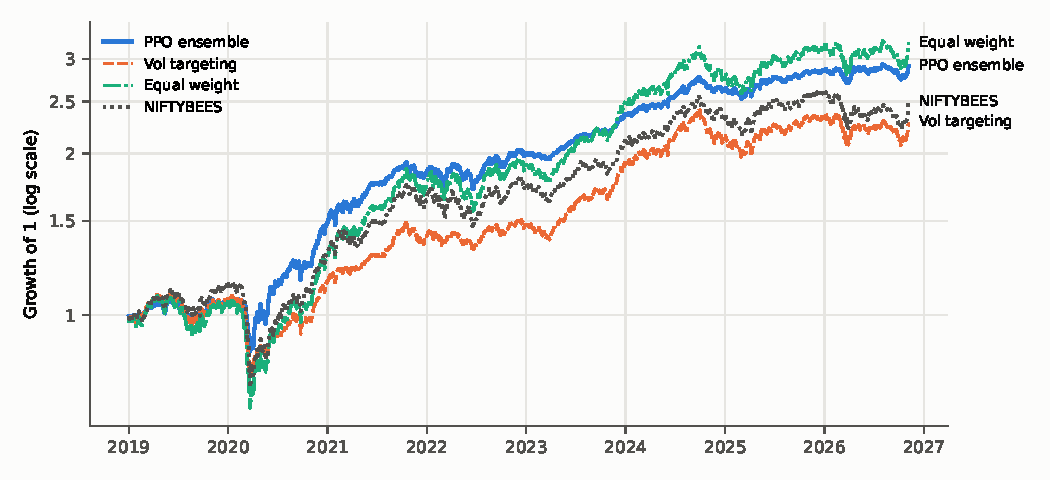
\includegraphics[width=\figwidth]{equity.pdf}
\caption{Growth of one rupee over the test path, log scale.}
\label{fig:equity}
\end{figure}

\begin{figure}[t]
\centering
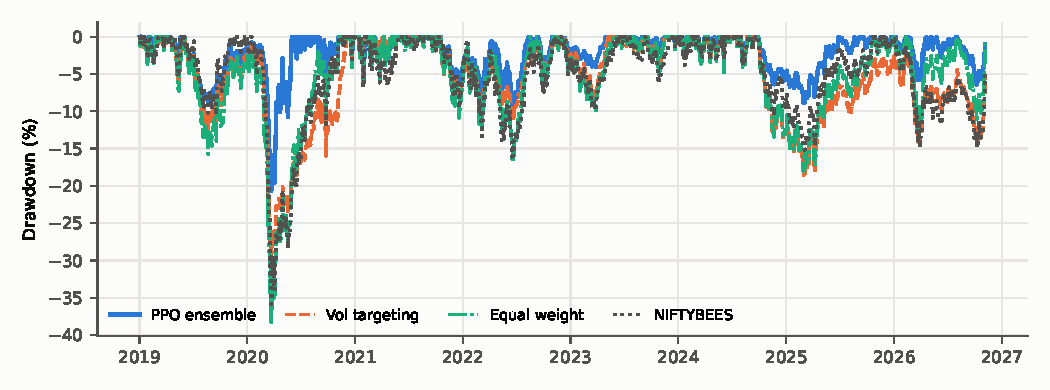
\includegraphics[width=\figwidth]{drawdown.pdf}
\caption{Drawdown from the running peak.}
\label{fig:drawdown}
\end{figure}

Table~\ref{tab:vs} sets the ensemble against every baseline. Apart from H1, these comparisons are exploratory. Apart from the two volatility-targeting rules, every interval includes zero: against equal weight the difference is \DvsEW{} \DvsEWCI{}, against NIFTYBEES \DvsBees{} \DvsBeesCI{}, and against risk parity at 0.7 exposure, the fixed exposure nearest the ensemble's average, \DvsRpB{} \DvsRpBCI{}. Volatility targeting's Sharpe ratio, \SRvt{}, is below that of risk parity at every fixed exposure (\SRrpA{} to \SRrpD{}).

\begin{table}[t]
\centering\small
\caption{Sharpe difference, PPO ensemble minus each baseline, over the whole path. Only the first row is the pre-registered test; the last is the post-hoc rule of Section~\ref{sec:vixrule}.}
\label{tab:vs}
\gtab{tab_vs.tex}
\end{table}

\subsection{Year by year}

\begin{figure}[t]
\centering
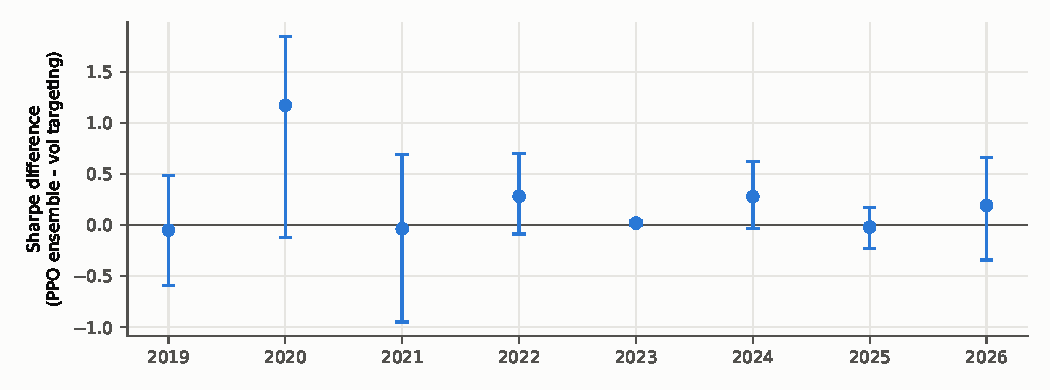
\includegraphics[width=\figwidth]{per_year_delta_sharpe.pdf}
\caption{Sharpe difference by test year, PPO ensemble minus volatility targeting, with 95\% bootstrap intervals.}
\label{fig:peryear}
\end{figure}

\begin{table}[t]
\centering\small
\caption{Sharpe ratio by test year. $^\dagger$Previously seen: our earlier work used these years.}
\label{tab:peryear}
\gtab{tab_per_year.tex}
\end{table}

The ensemble is ahead of volatility targeting in \NYearsAhead{} of the \NYears{} test years (Figure~\ref{fig:peryear}, Table~\ref{tab:peryear}), but no single year's interval excludes zero. The largest gap is 2020, at \DeltaTwenty{} \DeltaTwentyCI{}. That fold's checkpoints all had negative validation Sharpe ratios (\ValTwentyMin{} to \ValTwentyMax{}) on 2018--2019, yet its models produced the ensemble's best test year. In 2019 every risk-parity strategy and equal weight trailed NIFTYBEES, which weights stocks by market capitalisation.

\subsection{Robustness}

\begin{table}[t]
\centering\small
\caption{Pre-registered robustness checks: single seeds, execution one session late and costs doubled.}
\label{tab:robust}
\gtab{tab_robust.tex}
\end{table}

\begin{figure}[t]
\centering
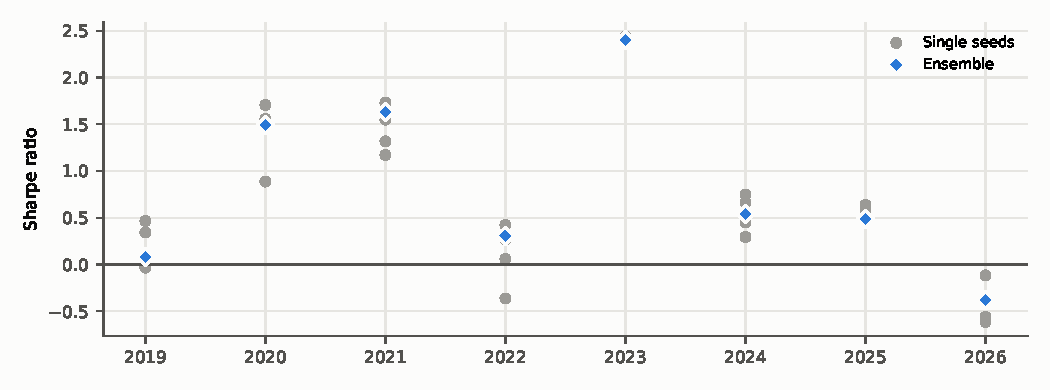
\includegraphics[width=\figwidth]{seed_spread.pdf}
\caption{Sharpe ratio by test year for each seed and for the ensemble.}
\label{fig:seeds}
\end{figure}

All \NSeedsBeatVT{} seeds beat volatility targeting on their own, with Sharpe ratios from \SRseedMin{} to \SRseedMax{} (Table~\ref{tab:robust}, Figure~\ref{fig:seeds}). Executing every trade one session late leaves the ensemble's Sharpe ratio at \SRppoLag{} (volatility targeting: \SRvtLag{}); an edge that relied on same-session information would shrink under the delay. With costs doubled to 20 basis points, the ensemble's Sharpe ratio is \SRppoCost{} and volatility targeting's \SRvtCost{}. The unfloored volatility rule scores \SRvtu{}. One hundred random policies over the same actions have a median Sharpe ratio of \SRrand{} and a 5th to 95th percentile range of \SRrandLo{} to \SRrandHi{}; the ensemble lies above that range.

The ensemble's daily Sharpe ratio is \SRdaily{}, with skewness \Skew{} and kurtosis \Kurt{}. With the single trial this study had run at the time of the test, its DSR is \DSRthis{}. Counting all \DSRpriorN{} trials in the ledger, including those of our earlier work, it is \DSRprior{}. After the post-hoc rule of Section~\ref{sec:vixrule}, which we count as a trial, the figures are \DSRnow{} (\DSRnowN{} trials) and \DSRpriorNow{} (\DSRpriorNowN{} trials).

\subsection{Drawdown episodes}

\begin{table}[t]
\centering\small
\caption{Return from peak to trough over NIFTYBEES drawdown windows. The protocol fixed the deepest windows whose peaks fall in 2020 and 2025; the other rows are the deepest on the whole path not already listed (exploratory).}
\label{tab:episodes}
\gtab{tab_episodes.tex}
\end{table}

The protocol fixed two windows: NIFTYBEES's deepest fall whose peak lies in 2020, and the same for 2025 (Table~\ref{tab:episodes}). From \EpiPeak{} to \EpiTrough{}, the ensemble lost \EpiPPO{}, against \EpiVT{} for volatility targeting, \EpiEW{} for equal weight and \EpiBees{} for NIFTYBEES. The 2025 window turned out to be a small dip (\EpiTwentyFiveBees{} for NIFTYBEES), because the larger 2024--25 correction peaked in September 2024. Over that correction, from \DeepThreePeak{} to \DeepThreeTrough{}, the ensemble lost \DeepThreePPO{}, against \DeepThreeVT{} for volatility targeting and \DeepThreeBees{} for NIFTYBEES.

\section{Exploratory analyses}\label{sec:exploratory}

Everything in this section was decided after the test run. Each analysis is recorded in the ledger, and none can change the verdict on H1.

\subsection{What the agent learned}

\begin{figure}[t]
\centering
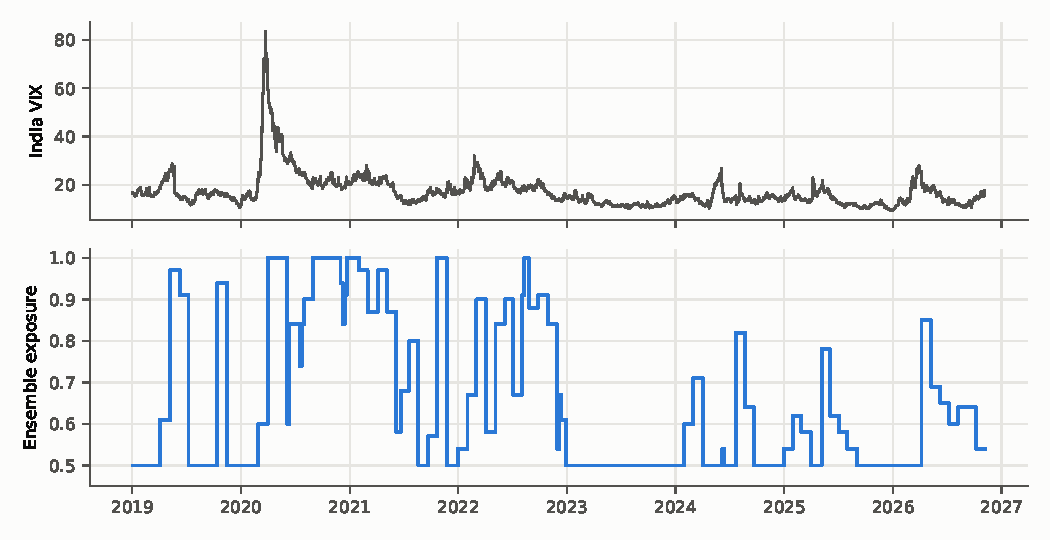
\includegraphics[width=\figwidth]{exposure_vs_vix.pdf}
\caption{India VIX (top) and the exposure chosen by the PPO ensemble (bottom), held from each decision to the next.}
\label{fig:vix}
\end{figure}

\begin{table}[t]
\centering\small
\caption{The ensemble's decisions grouped by India VIX at the decision (exploratory).}
\label{tab:buckets}
\gtab{tab_vix_buckets.tex}
\end{table}

Across its \NDecisions{} decisions, the ensemble's chosen exposure correlates \CorrVix{} with India VIX at the decision and \CorrDD{} with the Nifty~50 drawdown from its 252-session high (Figure~\ref{fig:vix}, Table~\ref{tab:buckets}). With VIX below 15 its mean exposure was \ExpLowVix{}, at the floor in \FloorShareLowVix{} of decisions; with VIX at 25 or above it was \ExpHighVix{}. The agent learned to hold little in calm markets and more after fear spikes. Volatility targeting does the reverse by construction, and its 60-session volatility estimate keeps exposure at the floor while a spike remains in the window.

The 2020 crash shows the difference. The ensemble's decisions were \CrashDecisions{}. It held half to 60 per cent of the portfolio through the fall and moved to full exposure eight days after the index bottomed on \EpiTrough{}, before most of the recovery.

\subsection{How much rests on 2020}

\begin{table}[t]
\centering\small
\caption{Sharpe differences by period, PPO ensemble minus each baseline, with the H1 bootstrap settings (exploratory). Seen: previously seen years.}
\label{tab:splits}
\gtab{tab_splits.tex}
\end{table}

Without 2020, the ensemble's lead over volatility targeting falls to \ExNoDelta{}, with a 5th percentile of \ExNoPfive{} (Table~\ref{tab:splits}). On the previously seen years 2022 to 2026 it is \ExSeenDelta{} (5th percentile \ExSeenPfive{}). On 2019 to 2021, the years our earlier work never used, it is \ExUnseenDelta{} (5th percentile \ExUnseenPfive{}), but that window contains 2020. Outside 2020, monthly equal weight has a higher Sharpe ratio than the ensemble (\ExNoEW{} against \ExNoPPO{}).

\subsection{A VIX threshold rule}\label{sec:vixrule}

\begin{table}[t]
\centering\small
\caption{The post-hoc VIX threshold rule against the PPO ensemble and volatility targeting, by period. ``First'' and ``second'' are the two strategies of each comparison, in order. Seen: previously seen years.}
\label{tab:vixrule}
\gtab{tab_vix_rule.tex}
\end{table}

To ask whether the agent does more than buy after VIX spikes, we designed one rule after the test, committed it to the repository before running it, recorded it in the ledger before it touched any test year, and count it as a trial. The rule holds full exposure when India VIX at the decision close is at or above a threshold and the 0.5 floor otherwise; the threshold (15, 20 or 25) and horizon (5 or 21 sessions) are chosen per fold on validation, like the other tuned baselines.

The rule's Sharpe ratio is \VRsr{} (Table~\ref{tab:vixrule}). The ensemble's lead over it is \VRdelta{}, with a 95\% interval of \VRci{}, so the two cannot be told apart; the rule's own lead over volatility targeting, \VRvsVT{} \VRvsVTci{}, is not significant either. Outside 2020 the rule is ahead of the ensemble (\VRnoRule{} against \VRnoPPO{}); in 2020 the ensemble is ahead (\VRtwentyPPO{} against \VRtwentyRule{}). Between January and April 2020 the two made their \NCrashDates{} decisions on the same dates and differed once: on \CrashDiffDate{}, with India VIX at \VixCrash{}, the rule moved to exposure \VRCrashExp{} and the ensemble to \PPOCrashExp{}. The rule's maximum drawdown is \VRmdd{}. Their exposures correlate \VRcorr{} session by session, so the ensemble is not simply this rule; but most of its measured edge over the rule comes from 2020, where the two policies differ by a single decision.

\section{Discussion}\label{sec:discussion}

\paragraph{What the evidence supports.} The registered hypothesis passed, with little room: the bootstrap 5th percentile is \HiPfive{} and the lower end of the two-sided interval is zero. Volatility targeting proved a weak comparator in this sample, below every fixed-exposure risk-parity portfolio, consistent with the out-of-sample findings of \citet{cederburg2020}. Against the passive baselines the ensemble's Sharpe advantage is not significant, though its drawdowns are clearly shallower. The deflated Sharpe ratio depends on how trials are counted: \DSRnow{} for this study alone and \DSRpriorNow{} once our earlier attempts are included. We think the second number is the honest one, and we encourage other RL studies to count trials across a project's history, not only within its final paper.

\paragraph{What the agent learned.} The agent learned contrarian volatility timing: low exposure in calm markets and high exposure after fear spikes. This is consistent with evidence that high implied volatility and variance risk premia precede higher equity returns \citep{whaley2000,bollerslev2009}, but our sample cannot separate a risk premium from the particular sequence of crashes and recoveries in 2019--2026. One V-shaped crash supplies most of the margin. A policy that buys after spikes is rewarded by quick recoveries and would be punished by slow, deep declines, of which the test path has none. A simple rule captures much of the behaviour; the agent's distinct contribution over that rule is not established.

\paragraph{Limitations.} The test covers one market and index over eight years, five of them previously seen. Six index members, among them HDFC until July 2023, have no price series and are excluded while members. Prices come from a public vendor; we repaired the errors we found, and the session calendar omits a few exchange sessions. Costs are proportional, without market impact or taxes. The exposure floor of 0.5, shared by the agent and volatility targeting, limits downside protection by design. To fit a one-week build we fixed the drawdown penalty at $\kappa=1$ and dropped an A2C comparison and a test on the Nifty Next~50; the ledger records these choices. The analyses of Section~\ref{sec:exploratory} were chosen after seeing the test results.

\paragraph{What would change the conclusion.} The decisive next test is the same frozen pipeline on a fresh universe, such as the Nifty Next~50, with the VIX threshold rule registered in advance as a comparator, and on a longer history that includes slow bear markets such as 2008.

\section{Conclusion}

Moving an RL agent from return forecasting to risk control turned a clear loss into a narrow pre-registered win over volatility targeting on point-in-time Nifty~50 equities. The win is real under the registered test but concentrated in 2020, and what the agent learned, raising exposure after fear spikes, is largely available from a two-parameter rule. We report it as such. Code, data hashes, the protocol, the trial ledger and every number in this paper are available in the project repository.\footnote{\url{https://github.com/eshentials/Deep-RL-For-Dynamic-Portfolio-Strategy}, branch \texttt{risk-budget-controller}; protocol tag \texttt{protocol-v1}.}

% TODO(authors): author contributions; acknowledgements; use of AI tools, as required by the venue.

\bibliographystyle{plainnat}
\bibliography{refs}

\appendix

\section{Folds and per-fold selections}\label{app:folds}

\begin{table}[H]
\centering\small
\caption{Walk-forward folds. The PPO column is the mean over five seeds of the best validation Sharpe ratio. Volatility targeting, the best fixed action and the post-hoc VIX rule were each chosen on the same validation years. $^\dagger$Previously seen.}
\gtab{tab_folds.tex}
\end{table}

\section{Trial ledger}\label{app:ledger}

\begin{table}[H]
\centering\small
\caption{Rows of \texttt{ledger.csv}. ``Trials counted'' is what enters the deflated Sharpe ratio. Development checks reran the registered configuration on fold 2019's training and validation years only and are not counted.}
\gtab{tab_ledger.tex}
\end{table}

\section{Data repairs}\label{app:data}

\begin{table}[H]
\centering\small
\caption{Corporate-action repairs. Demergers use the exchange's special pre-open discovered price; the split artifact is a vendor adjustment at a year boundary.}
\gtab{tab_repairs.tex}
\end{table}

\end{document}
